\chapter{Resultados Preliminares}
\label{ch:03-results}

“Language, never forget, is more fashion than science, and matters of usage, spelling and pronunciation tend to wander around like hemlines.” 
― Bill Bryson, The Mother Tongue: English and How It Got That Way

\section{Rede FFD}
\label{sec:ffd}

\subsection{Modelo}
\subsection{Corpus}
\subsection{Resultados}

\section{Encoder-Decoder}
\label{sec:seq2seq}

Como discutido na Seção \ref{sec:enc-dec}, os modelos do tipo Encoder-Decoder parecem promissores para o alcance dos objetivos propostos. Nessa seção são discutidos e comparados alguns testes que exibem a mesma arquitetura (Fig. \ref{fig:encdec}), porém alteram-se alguns dos hiperparâmetros possíveis e testam-se também diferentes corpora.

As amostras de treinamento foram subdivididas entre treino (80\%) e validação (20\%). Essa partição tem como objetivo avaliar o modelo quanto a predições em dados novos. Resultados de predições sobre alguns verbos de teste são exibidos no Apêndice.
%incluir ref Keras

\begin{figure}[h]
  \centering
  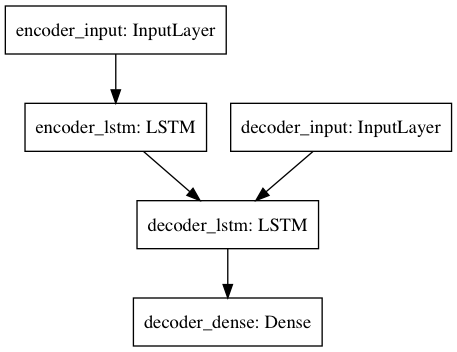
\includegraphics[width=0.5\linewidth]{img/draw-model6.png}
  \caption{Arquitetura Encoder-Decoder Desenvolvida}
  \label{fig:encdec}
\end{figure}

\subsection{Modelo Encoder-Decoder 1} 

\subsubsection{Corpus}
Esse modelo foi treinado na mesma base apresentada na Seção %ref tal.

\subsubsection{Hiperparâmetros} 

\begin{table}[h]
\centering
\begin{tabular}{ll}
Numero de Amostras Treinamento: & 325 \\
Numero de Amostras Teste: & 100 \\
Numero de tokens unicos do Input: & 22 \\
Numero de tokens unicos do Output: & 26 \\
Comprimento maximo da sequencia para inputs: & 11 \\
Comprimento maximo da sequencia para outputs: & 13 \\
Custo: & categorical\_crossentropy \\
Optimizador & rmsprop \\
Ativação & softmax \\
Épocas & 130 \\
Batch Size & 64
\end{tabular}
\caption{Tabela Resumo Estrutural do Modelo Encoder-Decoder 1}
\label{tab:res1}
\end{table}

\subsubsection{Resultados}

\begin{figure}[h]
  \centering
  \begin{subfigure}[b]{0.45\linewidth}
    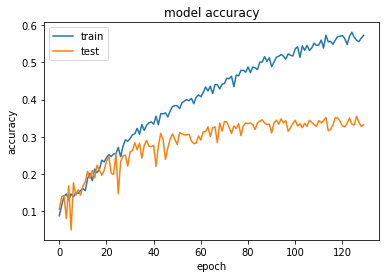
\includegraphics[width=\linewidth]{img/enc-dec-1.png}
    \caption{Resultados de Acurácia por Época}
  \end{subfigure}
  \begin{subfigure}[b]{0.45\linewidth}
    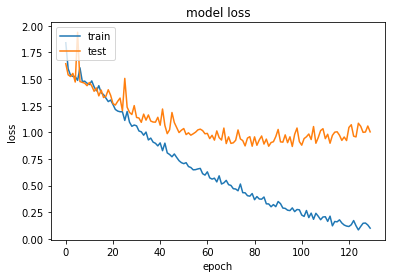
\includegraphics[width=\linewidth]{img/enc-dec-1-loss.png}
    \caption{Resultados de Custo por Época}
  \end{subfigure}
  \caption{Gráficos dos Resultados do Modelo}
  \label{fig:plots1}
\end{figure}

\begin{table}[h]
\centering
\begin{tabular}{llllll}
\textbf{Best Epoch Score} & \textbf{Val\_Acc} & \textbf{Vall\_Loss} & \textbf{Loss} & \textbf{Acc} & \textbf{Time} \\
97 & 0.342 & 0.867 & 0.290 & 0.508 & 2 min
\end{tabular}
\caption{Scores do Modelo Encoder-Decoder 1}
\label{tab:res-enc-dec-1}
\end{table}

\subsubsection{Discussão}



\subsection{Modelo Encoder-Decoder 2}
%Falar que eu quis testar o corpus com 55% de irregulares q foi oq teve melhor acuracia no ffd 

\subsubsection{Corpus}

\subsubsection{Hiperparâmetros} 

\begin{table}[h]
\centering
\begin{tabular}{ll}
Numero de Amostras Treinamento: & 452 \\
Numero de Amostras Teste: & 21 \\
Numero de tokens unicos do Input: & 23 \\
Numero de tokens unicos do Output: & 27 \\
Comprimento maximo da sequencia para inputs: & 13 \\
Comprimento maximo da sequencia para outputs: & 15 \\
Custo: & categorical\_crossentropy \\
Optimizador & rmsprop \\
Ativação & softmax \\
Épocas & 150 \\
Batch Size & 64
\end{tabular}
\caption{Tabela Resumo Estrutural do Modelo Encoder-Decoder 2}
\label{tab:res1}
\end{table}

\subsubsection{Resultados}

\begin{figure}[h]
  \centering
  \begin{subfigure}[b]{0.45\linewidth}
    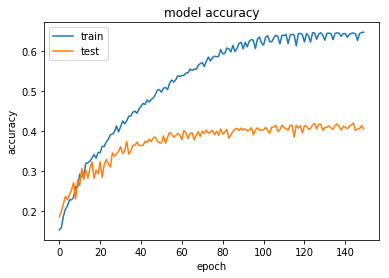
\includegraphics[width=\linewidth]{img/enc-dec-2.png}
    \caption{Resultados de Acurácia por Época}
  \end{subfigure}
  \begin{subfigure}[b]{0.45\linewidth}
    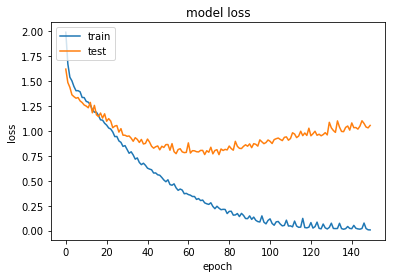
\includegraphics[width=\linewidth]{img/enc-dec-2-loss.png}
    \caption{Resultados de Custo por Época}
  \end{subfigure}
  \caption{Gráficos dos Resultados do Modelo}
  \label{fig:plots2}
\end{figure}

\begin{table}[h]
\centering
\begin{tabular}{llllll}
\textbf{Best Epoch Score} & \textbf{Val\_Acc} & \textbf{Vall\_Loss} & \textbf{Loss} & \textbf{Acc} & \textbf{Time} \\
145 & 0.419 & 1.048 & 0.014 & 0.644 & 4 min
\end{tabular}
\caption{Scores do Modelo Encoder-Decoder 2}
\label{tab:res-enc-dec-2}
\end{table}

\subsubsection{Discussão}

\subsection{Modelo Encoder-Decoder 3}
%Falar que eu quis aumentar a amostra pra ver se melhorava as coisas

\subsubsection{Corpus}
\subsubsection{Hiperparâmetros} 

\begin{table}[h]
\centering
\begin{tabular}{ll}
Numero de Amostras Treinamento: & 2000 \\
Numero de Amostras Teste: & 100 \\
Numero de tokens unicos do Input: & 26 \\
Numero de tokens unicos do Output: & 32 \\
Comprimento maximo da sequencia para inputs: & 15 \\
Comprimento maximo da sequencia para outputs: & 16 \\
Custo: & categorical\_crossentropy \\
Optimizador & rmsprop \\
Ativação & softmax \\
Épocas & 100 \\
Batch Size & 64
\end{tabular}
\caption{Tabela Resumo Estrutural do Modelo Encoder-Decoder 3}
\label{tab:res3}
\end{table}

\subsubsection{Resultados}
%falar q eu adicionei dropout e explicar oq é isso

\begin{figure}[h]
  \centering
  \begin{subfigure}[b]{0.45\linewidth}
    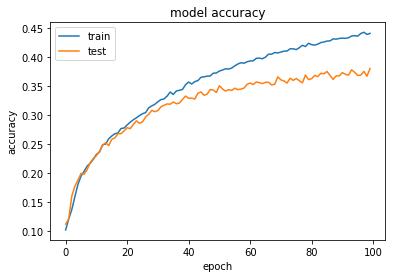
\includegraphics[width=\linewidth]{img/enc-dec-3.png}
    \caption{Resultados de Acurácia por Época}
  \end{subfigure}
  \begin{subfigure}[b]{0.45\linewidth}
    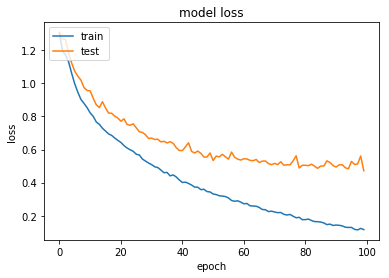
\includegraphics[width=\linewidth]{img/enc-dec-3-loss.png}
    \caption{Resultados de Custo por Época}
  \end{subfigure}
  \caption{Gráficos dos Resultados do Modelo}
  \label{fig:plots3}
\end{figure}

\begin{table}[h]
\centering
\begin{tabular}{llllll}
\textbf{Best Epoch Score} & \textbf{Val\_Acc} & \textbf{Vall\_Loss} & \textbf{Loss} & \textbf{Acc} & \textbf{Time} \\
100 & 0.380 & 0.471 & 0.115 & 0.440 & 11 min
\end{tabular}
\caption{Scores do Modelo Encoder-Decoder 3}
\label{tab:res-enc-dec-3}
\end{table}

\subsubsection{Discussão}
%Vale comentar aqui que eu tambem testei uma outra com recurrent dropout e nao deu certo

\subsection{Modelo Encoder-Decoder 4}
%Falar que eu quis mudar a funcao de ativacao pra ver oq acontecia e o otimizador tb (deve ter tido uma razao pra eu ter feito isso, deve ta no deep learning la)
\subsubsection{Corpus}
\subsubsection{Hiperparâmetros} 

\begin{table}[h]
\centering
\begin{tabular}{ll}
Numero de Amostras Treinamento: & 2000 \\
Numero de Amostras Teste: & 100 \\
Numero de tokens unicos do Input: & 26 \\
Numero de tokens unicos do Output: & 29 \\
Comprimento maximo da sequencia para inputs: & 15 \\
Comprimento maximo da sequencia para outputs: & 16 \\
Custo: & categorical\_crossentropy \\
Optimizador & adam \\
Ativação & relu \\
Épocas & 100 \\
Batch Size & 64
\end{tabular}
\caption{Tabela Resumo Estrutural do Modelo Encoder-Decoder 4}
\label{tab:res4}
\end{table}

\subsubsection{Resultados}
%falar q eu adicionei dropout e explicar oq é isso

\begin{figure}[h]
  \centering
  \begin{subfigure}[b]{0.45\linewidth}
    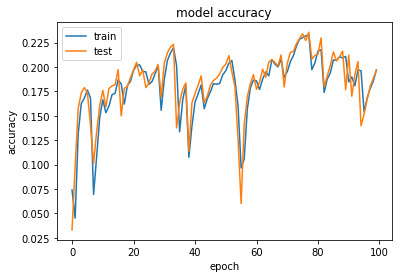
\includegraphics[width=\linewidth]{img/enc-dec-4.png}
    \caption{Resultados de Acurácia por Época}
  \end{subfigure}
  \begin{subfigure}[b]{0.45\linewidth}
    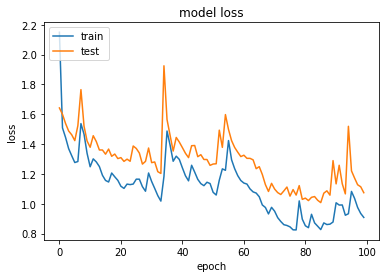
\includegraphics[width=\linewidth]{img/enc-dec-4-loss.png}
    \caption{Resultados de Custo por Época}
  \end{subfigure}
  \caption{Gráficos dos Resultados do Modelo}
  \label{fig:plots4}
\end{figure}

\begin{table}[h]
\centering
\begin{tabular}{llllll}
\textbf{Best Epoch Score} & \textbf{Val\_Acc} & \textbf{Vall\_Loss} & \textbf{Loss} & \textbf{Acc} & \textbf{Time} \\
86 & 0.210 & 1.00 & 0.820 & 0.207 & 10 min
\end{tabular}
\caption{Scores do Modelo Encoder-Decoder 4}
\label{tab:res-enc-dec-4}
\end{table}

\subsubsection{Discussão}
%ficou uma bosta
 
 \subsection{Modelo Encoder-Decoder 5}
%Falar que eu quis aumentar mais ainda a amostra

\subsubsection{Corpus}
\subsubsection{Hiperparâmetros} 

\begin{table}[h]
\centering
\begin{tabular}{ll}
Numero de Amostras Treinamento: & 3000 \\
Numero de Amostras Teste: & 100 \\
Numero de tokens unicos do Input: & 26 \\
Numero de tokens unicos do Output: & 32 \\
Comprimento maximo da sequencia para inputs: & 15 \\
Comprimento maximo da sequencia para outputs: & 16 \\
Custo: & categorical\_crossentropy \\
Optimizador & rmsprop \\
Ativação & softmax \\
Épocas & 100 \\
Batch Size & 64
\end{tabular}
\caption{Tabela Resumo Estrutural do Modelo Encoder-Decoder 5}
\label{tab:res5}
\end{table}

\subsubsection{Resultados}
%falar q eu ainda nao adicionei o dropout mas pode ser legal adicionar

\begin{figure}[h]
  \centering
  \begin{subfigure}[b]{0.45\linewidth}
    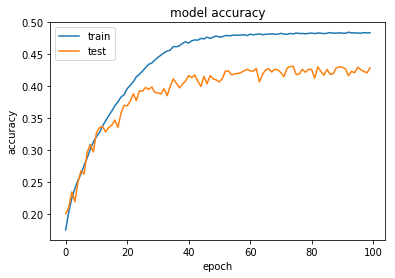
\includegraphics[width=\linewidth]{img/enc-dec-5.png}
    \caption{Resultados de Acurácia por Época}
  \end{subfigure}
  \begin{subfigure}[b]{0.45\linewidth}
    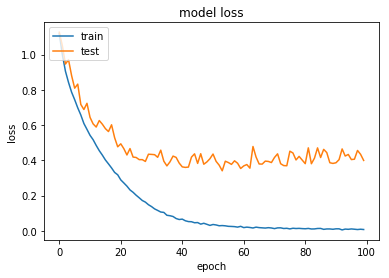
\includegraphics[width=\linewidth]{img/enc-dec-5-loss.png}
    \caption{Resultados de Custo por Época}
  \end{subfigure}
  \caption{Gráficos dos Resultados do Modelo}
  \label{fig:plots5}
\end{figure}

\begin{table}[h]
\centering
\begin{tabular}{llllll}
\textbf{Best Epoch Score} & \textbf{Val\_Acc} & \textbf{Vall\_Loss} & \textbf{Loss} & \textbf{Acc} & \textbf{Time} \\
54 & 0.423 & 0.340 & 0.030 & 0.4789 & 15 min
\end{tabular}
\caption{Scores do Modelo Encoder-Decoder 5}
\label{tab:res-enc-dec-5}
\end{table}

\subsubsection{Discussão}
%ficou promissor